%%%%%%%%%%%%%%%%%%%%%%%%%%%%%%%%%%%%%%%%%%%%%%%%%%%%%%%%%%%%%%%%%%%%%%
% 
% Benutzt Vorlage 
%
%%%%%%%%%%%%%%%%%%%%%%%%%%%%%%%%%%%%%%%%%%%%%%%%%%%%%%%%%%%%%%%%%%%%%%
%

\documentclass[11pt,a4paper]{article}
%\documentclass[conference]{IEEEtran}
\usepackage{epsfig}
\usepackage{amsthm, amssymb}
\usepackage[utf8]{inputenc}
\usepackage{color}
\usepackage[fleqn]{amsmath}
\usepackage{float,tikz}
\usepackage{amssymb, amsfonts, amsthm, booktabs,wasysym}
\usepackage[hidelinks]{hyperref}
\usepackage{verbatim}
\usepackage{tabularx}
\usepackage{graphicx}
\usepackage{longtable}
\usepackage{subcaption}
\usepackage[round]{natbib}


\newcommand{\fnurl}[2]{\footnote{\url{#1} (last accessed: #2)}} %URL als Fussnote
\newcommand{\TODO}[1]{{\color{red}\fbox{#1}}\PackageWarning{TODO}{**** TODO (page \thepage): #1 ****}}
\newcommand{\m}[1]{\begin{pmatrix} #1 \end{pmatrix}}
\newcommand{\lx}[1]{\lim_{n \rightarrow \infty} \left( #1 \right)}
\newcommand{\ml}[1]{\begin{multline*} #1 \\ \end{multline*}}
\newcommand{\sN}{\mathbb{N}}
\newcommand{\sR}{\mathbb{R}}
\newcommand{\folg}{\quad \ensuremath{\Rightarrow} \quad}
\newcommand{\ctbl}[2]{\begin{center}\begin{tabular}{#1} #2
\end{tabular}\end{center}}
\newcommand{\al}[1]{\begin{aligned} #1 \end{aligned}}
\newcommand{\alg}[1]{\begin{align*} #1 \end{align*}}
\newcommand{\equmf}{\quad \Leftrightarrow \quad}
\newcommand{\mpgv}[2]{\begin{minipage}{#1} \texttt{#2} \end{minipage}}
\newcommand{\includecode}[1]{{\footnotesize \begin{flushright} \texttt{#1}
  \end{flushright} \vspace{-2mm} \hrule \verbatiminput{#1} \hrule \vspace{5mm}}}
\newcommand{\todo}[1]{{\huge \\\color{red}  TODO: #1 }}
\newcommand{\block}[2]{\ensuremath{\underbrace{\left [ #1 \right ]}_{#2}}}
\renewcommand{\(}{\left (}
\renewcommand{\)}{\right )}


% correct bad hyphenation here
\hyphenation{ana-ly-sis net-work}

%
\begin{document}
\title{
  {\small Bioinformatics II 2015 \hfill project 3, \today}\\
   Atomic Contact Energies
}

\author{
Max Emil Schön, Adrian Geißler
}

% make the title area
\maketitle


%\begin{abstract}
%\end{abstract}


\section{Introduction}
The free energy functions needed to model Protein structures are made up of multiple components including van-der-Waals energies, electrostatics, dipole interactions, torsions and others. Here, we focus on atomic contact energies (ACE) of Proteins.\\
\cite{Zhang1997} describe a method to compute contact energies based on atoms rather than residue interactions, as proposed by \citet{Miyazawa1996}. 
\section{Material and Methods}
\subsection{Energy computation}\label{energies}
We implemented the Computation of atomic contact energies as proposed by \citet{Zhang1997}. Only heavy atoms were considered as potential pair members. We scanned every pair of atoms in a peptide chain for possible contact pairs. A contact pair is defined by \citet{Zhang1997} as two atoms that have a distance $\leq 6$\,\AA\ and are located at least ten bonds of the backbone away from each other. The bond distance criterion is implemented in terms of residues and the atoms' connectivity classes (Appendix in \citet{Zhang1997}). \\
For every valid contact pair an energy is given by Table 1 in \citet{Zhang1997}, which is based on the idea of grouping atoms into atom types with similar contact energy behaviour. As \citet{Zhang1997}, we used 18 atom types. To compute the overall energy of a given structure, we summed over all such contact pairs.
\subsection{Data}
The Critical Assessment of protein Structure Prediction (CASP) experiments\fnurl{http://www.predictioncenter.org/casp11}{\today} provides a variety of protein structure predictions from different researchers worldwide. We used 4 Protein targets (T0762, T0769, T0776, T0784) and the respective predictions from the current CASP11 experiment to test our energy computation from \ref{energies}.
\subsection{RMSD}
For the evaluation of the predicted structures we aligned the backbone C$\alpha$ atoms of the prediction with those of the target experimental structure \citep{pdb}. 


\section{Results}
\begin{figure}[!h]
	\begin{subfigure}{.5\textwidth}
		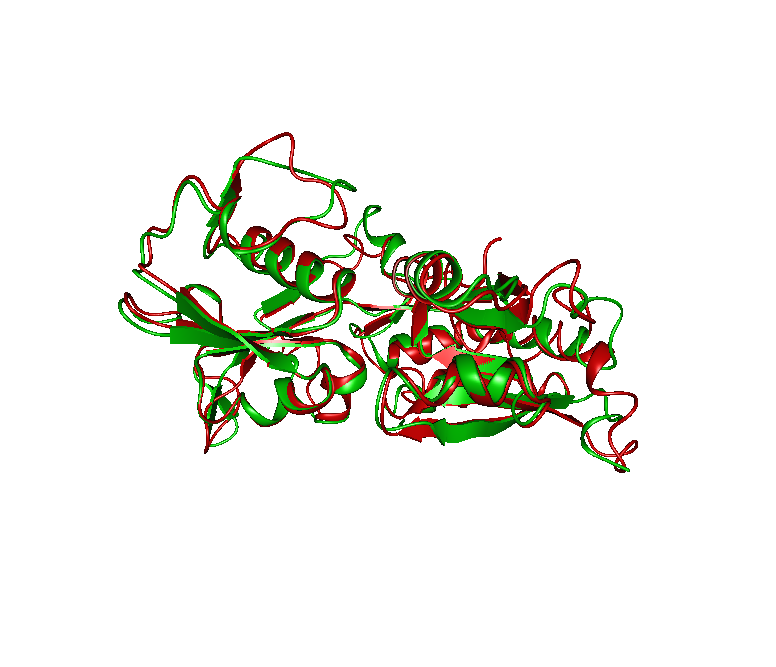
\includegraphics[width=\textwidth]{figures/T0762TS008}
		\subcaption{}
	\end{subfigure}
	\begin{subfigure}{.5\textwidth}
		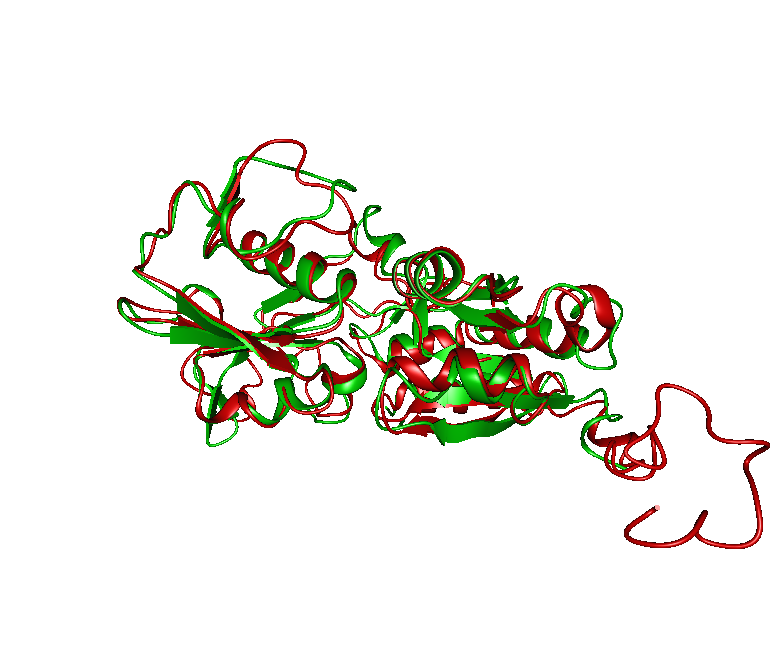
\includegraphics[width=\textwidth]{figures/T0762TS251}
		\subcaption{}
	\end{subfigure}
	 \caption{Best scoring predictions of T0762 evaluated using (a) atomic contact energies (008) and (b) the RMSD between prediction and experimental structure (251). Both predictions were visualized in BALLView \citep{ballview}. green: target experimental stucture. red: predicted structure.}
\end{figure}

\begin{figure}[!h]
	\begin{subfigure}{.5\textwidth}
		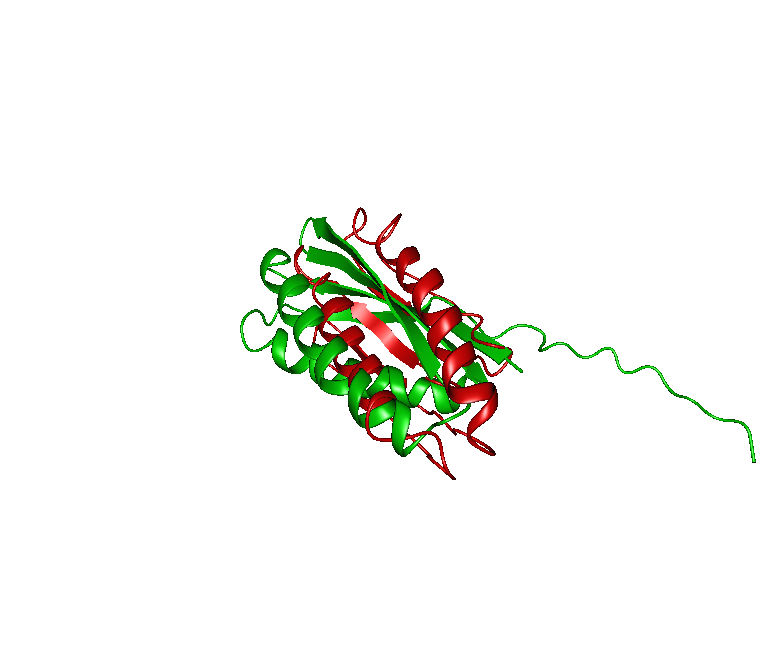
\includegraphics[width=\textwidth]{figures/T0769TS442}
		\subcaption{}
	\end{subfigure}
	\begin{subfigure}{.5\textwidth}
		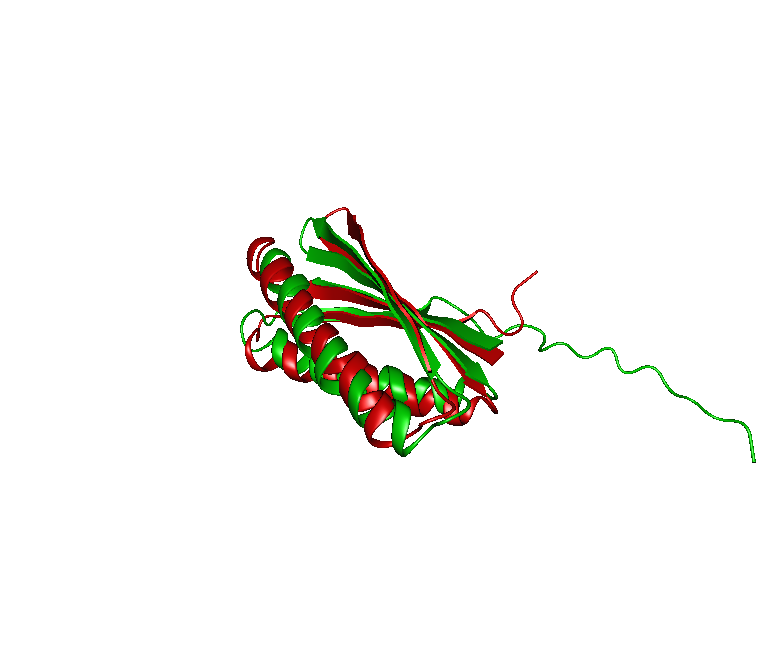
\includegraphics[width=\textwidth]{figures/T0769TS241}
		\subcaption{}
	\end{subfigure}
	 \caption{Best scoring predictions of T0769 evaluated using (a) atomic contact energies (442) and (b) the RMSD between prediction and experimental structure (241). Both predictions were visualized in BallView \citep{ballview}. green: target experimental stucture. red: predicted structure.}
\end{figure}

\begin{figure}[!h]
	\begin{subfigure}{.5\textwidth}
		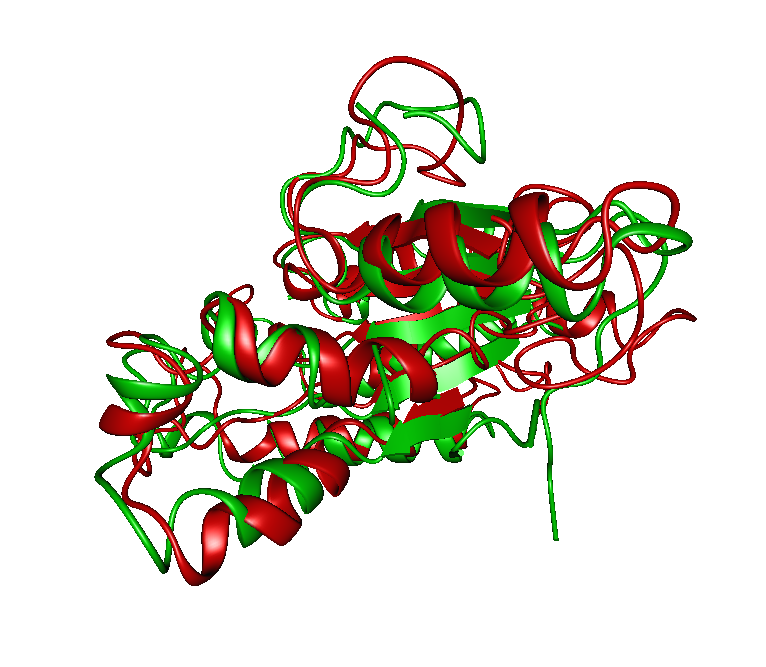
\includegraphics[width=\textwidth]{figures/T0776TS300}
		\subcaption{}
	\end{subfigure}
	\begin{subfigure}{.5\textwidth}
		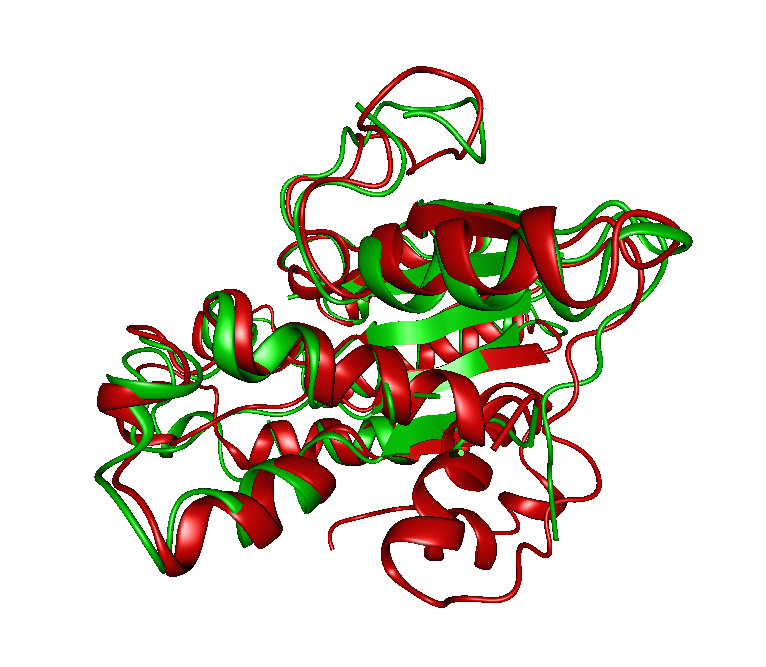
\includegraphics[width=\textwidth]{figures/T0776TS420}
		\subcaption{}
	\end{subfigure}
	 \caption{Best scoring predictions of T0776 evaluated using (a) atomic contact energies (300) and (b) the RMSD between prediction and experimental structure (420). Both predictions were visualized in BallView \citep{ballview}. green: target experimental stucture. red: predicted structure.}
\end{figure}

\begin{figure}[!h]
	\begin{subfigure}{.5\textwidth}
		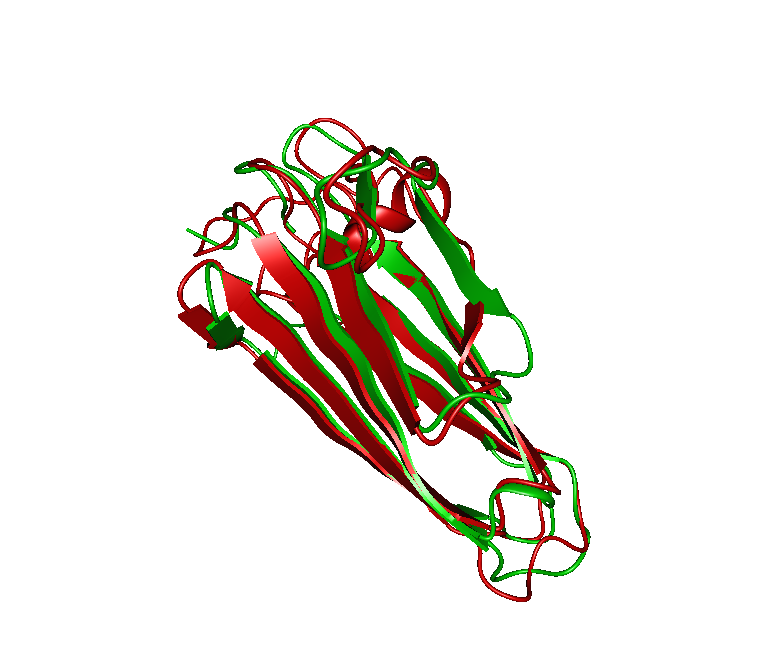
\includegraphics[width=\textwidth]{figures/T0784TS117}
		\subcaption{}
	\end{subfigure}
	\begin{subfigure}{.5\textwidth}
		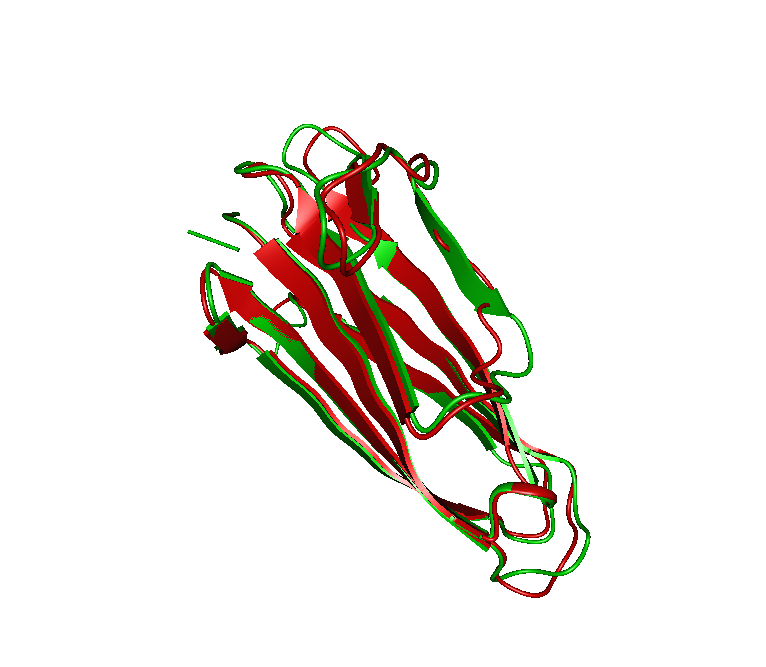
\includegraphics[width=\textwidth]{figures/T0784TS156}
		\subcaption{}
	\end{subfigure}
	\caption{Best scoring predictions of T0776 evaluated using (a) atomic contact energies (117) and (b) the RMSD between prediction and experimental structure (156). Both predictions were visualized in BallView \citep{ballview}. green: target experimental stucture. red: predicted structure.}
\end{figure}

\begin{figure}[!h]
	\begin{subfigure}{.5\textwidth}
		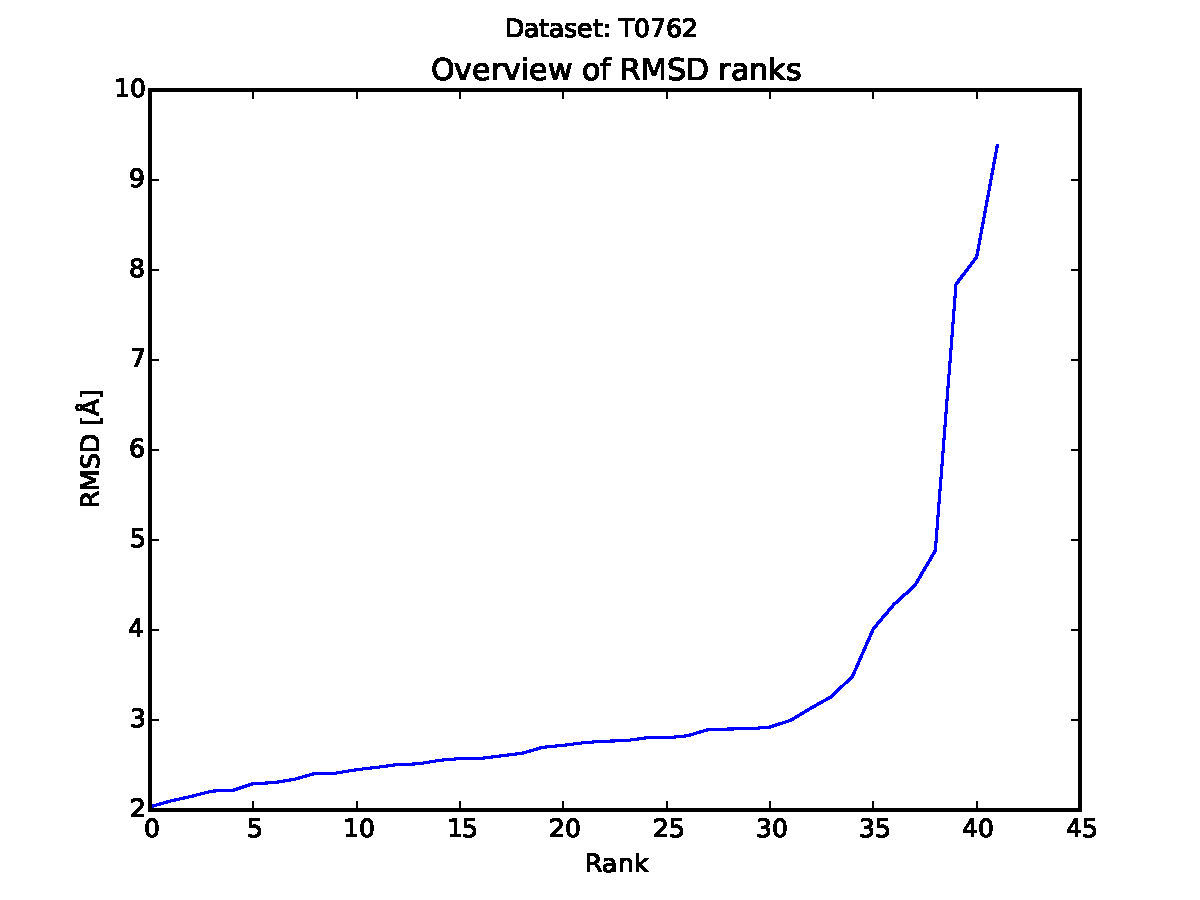
\includegraphics[width=\textwidth]{../results/rank_T0762}
		\subcaption{}
	\end{subfigure}
	\begin{subfigure}{.5\textwidth}
		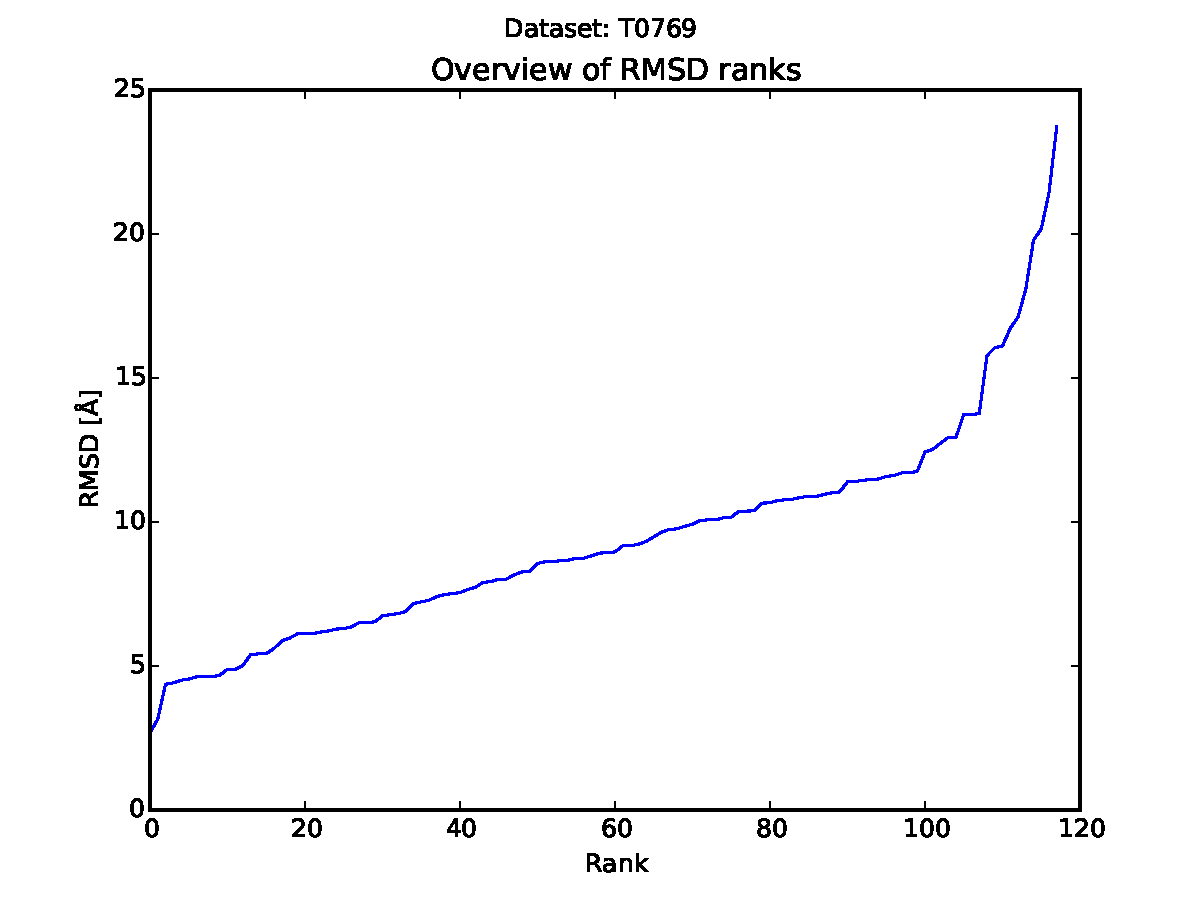
\includegraphics[width=\textwidth]{../results/rank_T0769}
		\subcaption{}
	\end{subfigure}
	\begin{subfigure}{.5\textwidth}
		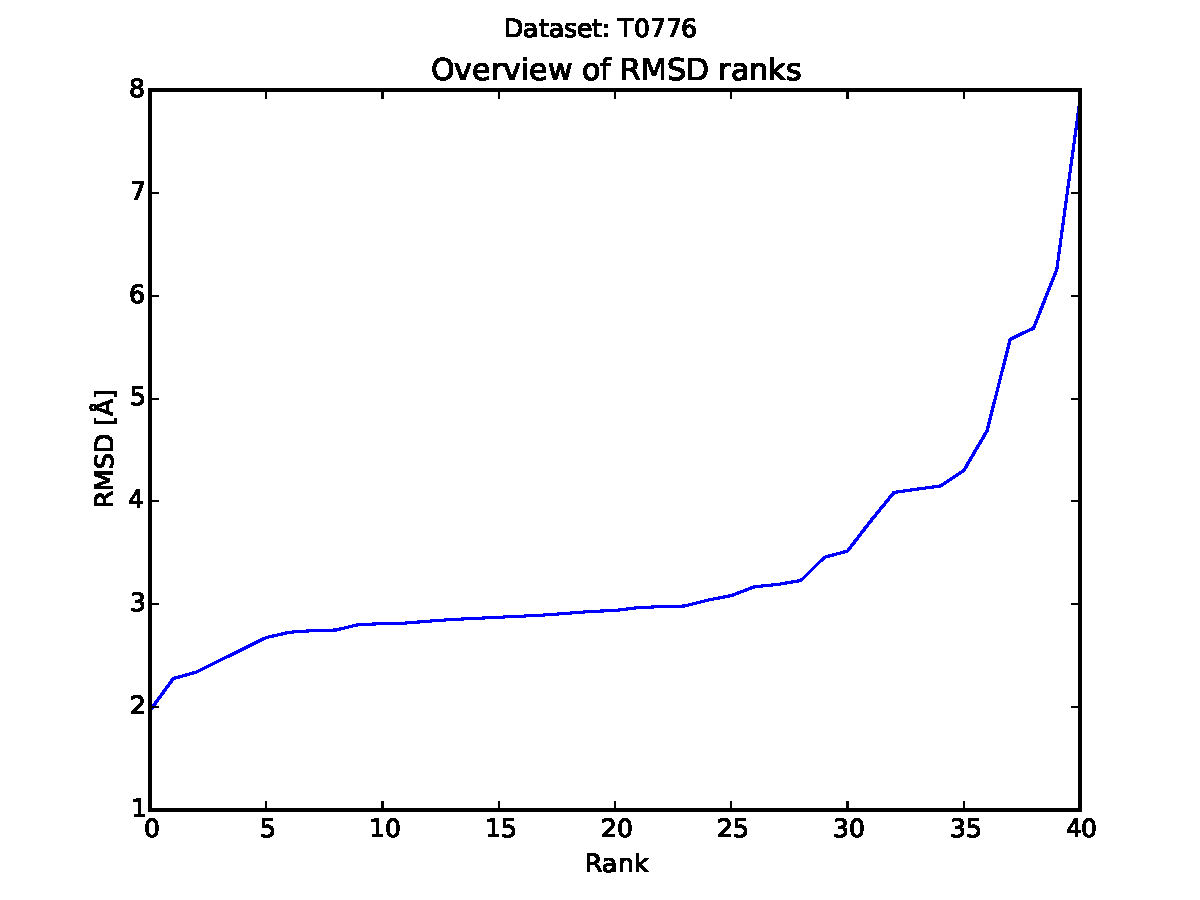
\includegraphics[width=\textwidth]{../results/rank_T0776}
		\subcaption{}
	\end{subfigure}
	\begin{subfigure}{.5\textwidth}
		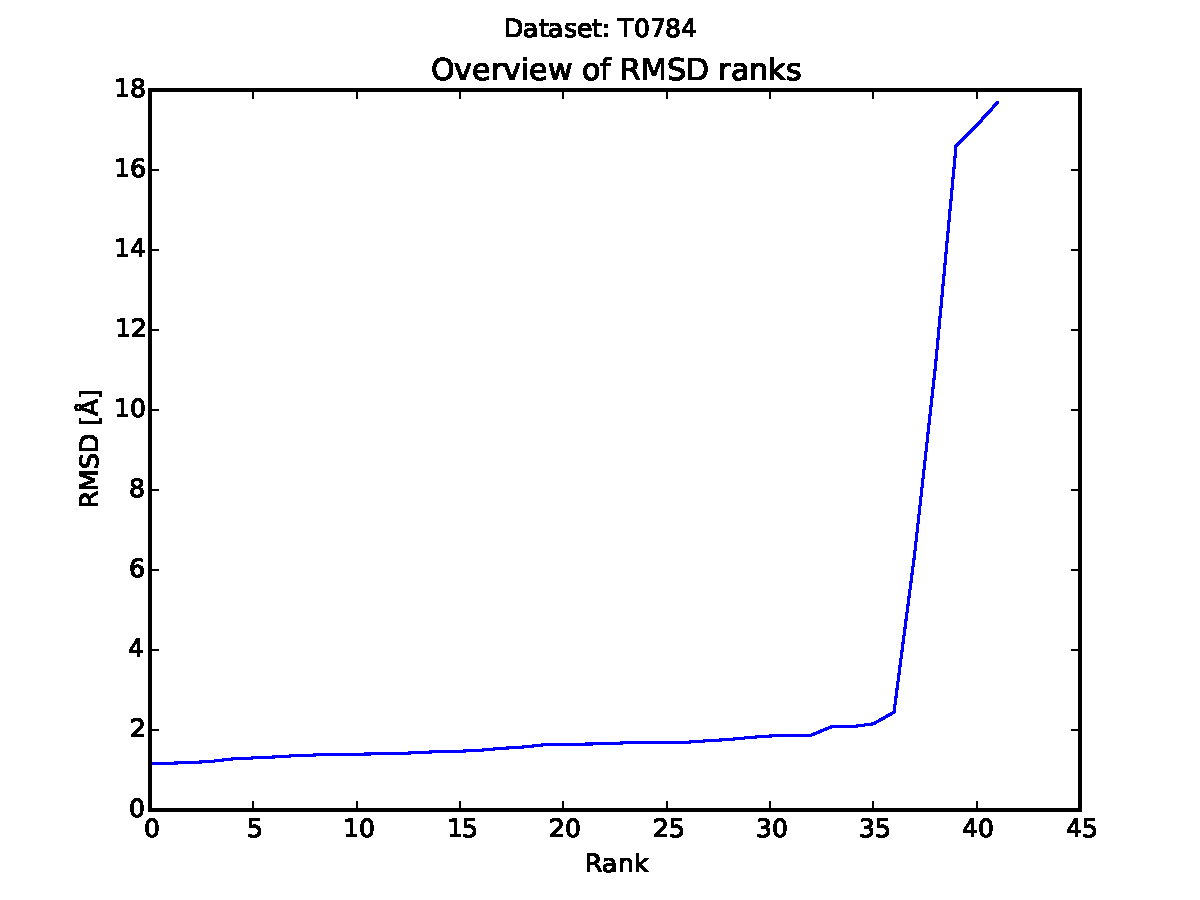
\includegraphics[width=\textwidth]{../results/rank_T0784}
		\subcaption{}
	\end{subfigure}
	\caption{RMSD VS. Rank in original CASP11 exeperiment. (a) T0762 (b) T0769 (c) T0776 (d) T0784}
\end{figure}

\section{Discussion}

%\begin{table}
\caption{results for predictions on T0762. Best energy and rmsd are marked in bold.}
\begin{tabular}{lll}
PDB & RMSD & Energy in kcal/mol\\\hline
T0762TS008\_1.pdb & 2.3423191305 & \textbf{-262.8469047619}\\
T0762TS011\_1.pdb & 2.7698841026 & -168.9030476191\\
T0762TS022\_1.pdb & 2.5058039439 & -162.9670952381\\
T0762TS038\_1.pdb & 2.5708829119 & -191.4314285714\\
T0762TS041\_1.pdb & 2.4066233264 & -247.9363333333\\
T0762TS050\_1.pdb & 2.9965283038 & -179.2812380952\\
T0762TS073\_1.pdb & 2.5517540142 & -180.0836666667\\
T0762TS117\_1.pdb & 2.7479596589 & -152.076952381\\
T0762TS133\_1.pdb & 2.4481363601 & -175.1629047619\\
T0762TS145\_1.pdb & 2.6966658285 & -126.8349047619\\
T0762TS156\_1.pdb & 2.3042503171 & -190.0696666667\\
T0762TS160\_1.pdb & 3.263572163 & -152.7326190476\\
T0762TS171\_1.pdb & 3.4890752584 & -138.0823809524\\
T0762TS184\_1.pdb & 2.2928815484 & -188.3076666667\\
T0762TS193\_1.pdb & 2.4744865096 & -174.6419047619\\
T0762TS206\_1.pdb & 3.134063264 & -144.5034285714\\
T0762TS210\_1.pdb & 2.5129260903 & -142.9043809524\\
T0762TS212\_1.pdb & 2.1513475418 & -166.0571904762\\
T0762TS216\_1.pdb & 2.4099770382 & -154.2829047619\\
T0762TS228\_1.pdb & 9.385668499 & -142.7432380952\\
T0762TS237\_1.pdb & 2.9223547684 & -169.5801428572\\
T0762TS251\_1.pdb & \textbf{2.0353168441} & -198.3766666667\\
T0762TS263\_1.pdb & 2.6020588681 & -168.0090476191\\
T0762TS268\_1.pdb & 2.8247720358 & -180.3427142857\\
T0762TS277\_1.pdb & 2.0999864471 & -160.3694285714\\
T0762TS279\_1.pdb & 2.8014960162 & -157.4457619048\\
T0762TS300\_1.pdb & 2.6303333034 & -186.3836190476\\
T0762TS335\_1.pdb & 4.4916672191 & -188.3896190476\\
T0762TS345\_1.pdb & 8.1449379541 & -187.4612380952\\
T0762TS346\_1.pdb & 2.8014960162 & -157.4457619048\\
T0762TS349\_1.pdb & 2.5729844986 & -176.5188095238\\
T0762TS381\_1.pdb & 4.0131846845 & -142.8844285714\\
T0762TS410\_1.pdb & 2.2182007065 & -162.9987142857\\
T0762TS414\_1.pdb & 4.2846602592 & -181.4261428572\\
T0762TS420\_1.pdb & 2.7646056492 & -171.873952381\\
T0762TS436\_1.pdb & 2.9020538844 & -165.2876190476\\
T0762TS448\_1.pdb & 2.8999667601 & -162.2623809524\\
T0762TS452\_1.pdb & 4.8824693376 & -187.9945714286\\
T0762TS454\_1.pdb & 7.8411398975 & -137.1416190476\\
T0762TS479\_1.pdb & 2.7188284869 & -159.5322857143\\
T0762TS492\_1.pdb & 2.8928415675 & -170.923\\
T0762TS499\_1.pdb & 2.2102185447 & -143.9080476191
\end{tabular}
\end{table}


\begin{longtable}{lll}
\caption{results on T079, best energy and rmsd are labeled in bold}
\endfirsthead PDB & RMSD & Energy in kcal/mol\\\hline
\endhead PDB & RMSD & Energy in kcal/mol\\\hline
T0769TS006\_1.pdb & 20.1730457219 & 9.9426666667\\
T0769TS008\_1.pdb & 7.656606437 & -47.6180952381\\
T0769TS011\_1.pdb & 7.90669551 & -53.1626666667\\
T0769TS014\_1.pdb & 7.2800902969 & -78.608047619\\
T0769TS022\_1.pdb & 6.2814170073 & -41.037047619\\
T0769TS024\_1.pdb & 8.1636320221 & -26.2007142857\\
T0769TS026\_1.pdb & 11.5847410454 & -11.5636190476\\
T0769TS032\_1.pdb & 11.0449515749 & -59.215047619\\
T0769TS034\_1.pdb & 12.4326106396 & -39.230047619\\
T0769TS038\_1.pdb & 11.4938620902 & -71.6676190476\\
T0769TS040\_1.pdb & 4.5479075741 & -75.5332857143\\
T0769TS041\_1.pdb & 7.1711046291 & -65.6891904762\\
T0769TS042\_1.pdb & 10.7702826637 & -76.5509047619\\
T0769TS044\_1.pdb & 10.379460472 & -84.324952381\\
T0769TS049\_1.pdb & 6.2149362872 & -46.1097619048\\
T0769TS050\_1.pdb & 8.9607134116 & -65.8122857143\\
T0769TS054\_1.pdb & 7.5130952377 & -67.1312380952\\
T0769TS056\_1.pdb & 10.0754920578 & -65.0741428571\\
T0769TS063\_1.pdb & 16.1141743491 & -67.052047619\\
T0769TS064\_1.pdb & 4.6211297931 & -66.2501904762\\
T0769TS065\_1.pdb & 9.4828543553 & -54.6042380952\\
T0769TS067\_1.pdb & 9.8518281632 & -11.4737619048\\
T0769TS073\_1.pdb & 10.7955344714 & -63.272\\
T0769TS080\_1.pdb & 9.6458158366 & -67.0588571429\\
T0769TS110\_1.pdb & 23.7304577067 & -16.3631904762\\
T0769TS111\_1.pdb & 9.7456809802 & -52.6412380952\\
T0769TS117\_1.pdb & 8.0170568464 & -59.8334761905\\
T0769TS118\_1.pdb & 5.8724940559 & -73.6708095238\\
T0769TS120\_1.pdb & 4.8855322705 & -69.8123333333\\
T0769TS132\_1.pdb & 12.7361139511 & -71.6454761905\\
T0769TS133\_1.pdb & 8.2845850564 & -63.7264761905\\
T0769TS144\_1.pdb & 8.6599310797 & -59.6228095238\\
T0769TS145\_1.pdb & 15.7795153686 & -9.5483333333\\
T0769TS155\_1.pdb & 17.1179459224 & -90.6197619048\\
T0769TS156\_1.pdb & 9.921559656 & -77.6414761905\\
T0769TS157\_1.pdb & 8.7380329701 & -60.2150952381\\
T0769TS160\_1.pdb & 9.1739726894 & -50.0969047619\\
T0769TS162\_1.pdb & 11.4072506411 & -69.2266666667\\
T0769TS169\_1.pdb & 10.388204067 & -81.0181904762\\
T0769TS171\_1.pdb & 9.7614822619 & -50.252047619\\
T0769TS173\_1.pdb & 16.0507642325 & -51.4058095238\\
T0769TS184\_1.pdb & 4.6211297931 & -66.2501904762\\
T0769TS186\_1.pdb & 4.5056666703 & -79.9672380952\\
T0769TS193\_1.pdb & 7.4138503031 & -34.809047619\\
T0769TS197\_1.pdb & 6.5098909593 & -75.0500952381\\
T0769TS203\_1.pdb & 6.1777008534 & -79.8995714286\\
T0769TS204\_1.pdb & 11.4452488091 & -57.5974761905\\
T0769TS210\_1.pdb & 9.3218468239 & -55.165\\
T0769TS212\_1.pdb & 10.6563858985 & -52.5722380952\\
T0769TS216\_1.pdb & 6.7414717331 & -72.8697142857\\
T0769TS228\_1.pdb & 10.7489144331 & -61.8762380952\\
T0769TS230\_1.pdb & 11.7064917635 & -71.1991904762\\
T0769TS235\_1.pdb & 10.3741848392 & -63.1856666667\\
T0769TS237\_1.pdb & 19.7873241656 & -25.9186190476\\
T0769TS241\_1.pdb & \textbf{2.6748016595} & -59.343047619\\
T0769TS251\_1.pdb & 11.4793688956 & -72.1082380952\\
T0769TS258\_1.pdb & 4.3658125828 & -74.3942380952\\
T0769TS260\_1.pdb & 7.5478941478 & -63.680952381\\
T0769TS263\_1.pdb & 6.3583017914 & -60.6837619048\\
T0769TS268\_1.pdb & 12.5206470774 & -59.0740952381\\
T0769TS276\_1.pdb & 9.2283590943 & -48.8672380952\\
T0769TS277\_1.pdb & 8.6187720319 & -66.4583809524\\
T0769TS279\_1.pdb & 7.9277072215 & -69.9848095238\\
T0769TS282\_1.pdb & 4.6205525448 & -65.9706666667\\
T0769TS290\_1.pdb & 8.6787419682 & -79.7527142857\\
T0769TS296\_1.pdb & 5.6087466103 & -58.6694285714\\
T0769TS300\_1.pdb & 10.8891677857 & -55.8492380952\\
T0769TS301\_1.pdb & 8.6187720319 & -66.4583809524\\
T0769TS310\_1.pdb & 6.7827244945 & -69.0379047619\\
T0769TS317\_1.pdb & 6.8894944503 & -80.6148095238\\
T0769TS322\_1.pdb & 6.1114435755 & -51.8862857143\\
T0769TS326\_1.pdb & 8.9346872229 & -66.206047619\\
T0769TS328\_1.pdb & 7.2269895599 & -68.7308095238\\
T0769TS333\_1.pdb & 5.9682157126 & -60.9969047619\\
T0769TS335\_1.pdb & 10.8604551953 & -64.507047619\\
T0769TS336\_1.pdb & 4.8855322705 & -69.8123333333\\
T0769TS338\_1.pdb & 13.758906479 & -69.6464285714\\
T0769TS342\_1.pdb & 6.1261436042 & -73.287047619\\
T0769TS345\_1.pdb & 9.1735222065 & -65.4832380952\\
T0769TS346\_1.pdb & 12.9339727638 & -34.0533333333\\
T0769TS347\_1.pdb & 8.7465818149 & -77.1880952381\\
T0769TS349\_1.pdb & 5.4210657112 & -55.3339047619\\
T0769TS357\_1.pdb & 12.9475028359 & -42.653\\
T0769TS358\_1.pdb & 13.7379987801 & -79.7847619048\\
T0769TS361\_1.pdb & 4.4147342409 & -79.04\\
T0769TS362\_1.pdb & 4.6812316055 & -64.3309047619\\
T0769TS364\_1.pdb & 10.0510151598 & -66.3444285714\\
T0769TS368\_1.pdb & 3.1590900898 & -66.7455238095\\
T0769TS381\_1.pdb & 10.9574952212 & -52.961047619\\
T0769TS386\_1.pdb & 21.4333289559 & -25.2683333333\\
T0769TS391\_1.pdb & 11.7579485804 & -44.0409047619\\
T0769TS403\_1.pdb & 6.2984516357 & -71.4070952381\\
T0769TS410\_1.pdb & 11.3970114047 & -49.1604285714\\
T0769TS414\_1.pdb & 11.0135831182 & -56.553952381\\
T0769TS417\_1.pdb & 10.148918345 & -40.8924285714\\
T0769TS420\_1.pdb & 8.8262360334 & -52.8872857143\\
T0769TS425\_1.pdb & 7.4797328656 & -58.3386666667\\
T0769TS428\_1.pdb & 5.0235525248 & -60.3364285714\\
T0769TS433\_1.pdb & 6.5335668605 & -76.7075714286\\
T0769TS434\_1.pdb & 8.0186462074 & -47.955047619\\
T0769TS436\_1.pdb & 5.4276048278 & -62.4596666667\\
T0769TS437\_1.pdb & 18.0746184973 & -31.9063809524\\
T0769TS438\_1.pdb & 10.1679787487 & -55.886047619\\
T0769TS439\_1.pdb & 7.7351910912 & -72.6902857143\\
T0769TS442\_1.pdb & 16.7228006464 & \textbf{-90.7309047619}\\
T0769TS445\_1.pdb & 6.5098909593 & -75.0500952381\\
T0769TS448\_1.pdb & 10.6652748317 & -65.3305238095\\
T0769TS452\_1.pdb & 10.8839209839 & -52.0201428571\\
T0769TS454\_1.pdb & 8.2663766022 & -36.2377619048\\
T0769TS457\_1.pdb & 6.817524943 & -70.8647619048\\
T0769TS465\_1.pdb & 8.5608396165 & -59.7923333333\\
T0769TS466\_1.pdb & 13.7327026472 & -31.1620952381\\
T0769TS476\_1.pdb & 6.1261436042 & -73.287047619\\
T0769TS479\_1.pdb & 11.6131435105 & -77.7516190476\\
T0769TS482\_1.pdb & 10.0754920578 & -65.0741428571\\
T0769TS483\_1.pdb & 11.7064917635 & -71.1991904762\\
T0769TS492\_1.pdb & 5.4000275617 & -66.2724285714\\
\end{longtable}

%bibliography
\bibliographystyle{abbrvnat}
% argument is your BibTeX string definitions and bibliography database(s)
\bibliography{ref}

\end{document}
